\chapter{Demonstrace použití knihovny}\label{chap:demonstration}

V této kapitole se zabývám demonstrací použití knihovny při testování. Ukázkové testy využívají průmyslový protokol ModbusTCP. 

\section{Nastavení knihovny}
Před započetím testování je potřeba provést prvotní nastavení testovací služby a testovaného zařízení.

\subsection{Příprava testovaného zařízení}
K použití testované knihovny na testovaném zařízení je potřeba implementovat rozhraní pro testované zařízení. Instance tohoto rozhraní následně musí být předána komponentě \inlinecode{TestRunner}. Implementace obou těchto částí je popsána v sekci \ref{sec:testrunner}. Komponenta \inlinecode{TestRunner} je následně inicializována za pomocí metody \inlinecode{Init} a následně je zavolána metoda \inlinecode{HandleInstructions}, která řídí testovací běh na zařízení.
 
\subsection{Testovací projekt}
Ke správě jednotlivých testů je potřeba vytvořit testovací projekt, ze kterého následně bude spouštěna testovací služba. Testovací projekt je vytvořen za pomocí IDE Visual Studio 2019, kde je využito předlohy nazvané \uv{Unit Test Project (.NET Framework)}.

Do tohoto projektu je následně přidán NuGet balíček, který obsahuje testovací knihovnu. Jelikož je knihovna uložena v Azure Artifacts, může být potřeba zároveň přidat Azure Artifacts jako zdroj NuGet balíčků. S instalací knihovny se přidá i složka \inlinecode{resources}, která obsahuje vše potřebné k nastavení testovací knihovny a testovací služby. Testovací projekt je následně uložen ve vlastním repositáři v Azure Repos.  

\subsubsection{Konfigurace}
Ve složce \inlinecode{resources} nalezneme soubor \inlinecode{config.xml}, který obsahuje konfiguraci služby. Tento soubor po zkopírování ze složky resource do kořenové složky projektu lze upravit do požadovaného základního nastavení. 

Testovací knihovna a služba očekává tento soubor v kořenové složce, ze které se spouští program. Soubor je tedy potřeba po kompilaci do této složky přesunout. Toho lze docílit za pomocí tzv. \uv{Post-build events}, neboli událostí po sestavení. Do těchto událostí je přidána direktiva, která po kompilaci, neboli sestavení, přesune konfigurační soubor do výstupní složky s programem. Tuto direktivu můžeme vidět na výpisu \ref{listing:postbuild}.

V tento moment je zároveň vhodné vytvořit soubor, ve kterém budou uloženy jednotlivé identifikátory testů. K tomu je využit soubor \inlinecode{TestEnumTemplate.cs.txt} ve složce \inlinecode{resources}. Jeho kopie je přesunuta mimo složku resources a následně je přejmenován na \inlinecode{TestEnum.cs}.

\begin{listing}[H]
    \centering
    \begin{cminted}[breaklines,stripnl=false]{text}

COPY "$(ProjectDir)config.xml"  "$(TargetDir)"
    \end{cminted}
\caption{Direktiva k přesunutí konfiguračního souboru}
\label{listing:postbuild}
\end{listing}

\section{Vytvoření testu}
Jednotlivé testy je potřeba implementovat pro všechny účastníky testování. Pro demonstraci funkcionality jsou vytvořeny dva testy:
\begin{enumerate}
    \item \inlinecode{MODD\_ADD\_CONF} -- Test, který otestuje přidání nastavení implementace protokolu ModbusTCP na testovaném zařízení.
    \item \inlinecode{MODD\_READ\_DATA} -- Test, při kterém se otestuje čtení z registrů na testovaném zařízení za pomoci osmi testovacích partnerů. Partneři budou číst z testovaného zařízení za pomoci protokolu ModbusTCP a následně kontrolovat správnost obdržených dat.
\end{enumerate}

Ke každému z testů je vytvořen stejnojmenný identifikátor v souboru \inlinecode{TestEnum.cs}.


\subsection{Testované zařízení}

Implementace testu \inlinecode{MODD\_ADD\_CONF} v první fázi nic neprovádí. Následně ve druhé fázi je testována metoda \inlinecode{mfd\_modd\_add\_configuration}, která vytváří konfigurace protokolu ModbusTCP. V poslední fázi jsou tyto konfigurace odstraněny.  

Implementaci testu \inlinecode{MODD\_READ\_DATA} lze vidět na výpisu \ref{listing:testcase_device}. Test v první fázi inicializuje protokol ModbusTCP a do výstupních registrů zapíše data. Jeden registr má velikost dva bajty. Během testovací fáze zařízení neprovádí žádné úkony. Zařízení nakonec vrací v poslední fázi testu do původního stavu před testováním.

Vytvořené testy jsou následně přidány do metody \inlinecode{getTest} v rozhraní pro testované zařízení. Metoda getTest musí po obdržení číselného identifikátoru jednotlivých testů vrátit instanci těchto testů.


\subsection{Testovací partner}
Implementace testu \inlinecode{MODD\_READ\_DATA}, kterou můžeme vidět na výpisu \ref{listing:testcase_partner} pro testovacího partnera je velmi obdobná implementaci pro testované zařízení. Implementace používá knihovnu EasyModbusTCP k vytvoření připojení s testovaným zařízením. 

Testovací partner v testovací fázi vytvoří připojení s testovaným zařízením a poté čte data z testovaného zařízení, které následně kontroluje s očekávanými daty. Tato implementace je součástí testovacího projektu. Test \inlinecode{MODD\_ADD\_CONF} nevyužívá testovacího partnera.


\subsection{Testovací služba}

K registraci testů pro testovací službu je použita standardní metodika vytváření testů dle frameworku MSTest, kterou můžeme vidět na výpisu \ref{listing:testcase_service}, kde lze vidět testovací třídu \inlinecode{Modbus} obsahující testovací metody \inlinecode{TestModdAddConf} a \inlinecode{TestModdReadData}. Třída i metody jsou označeny atributy definovanými frameworkem MSTest. 

Uvnitř testovací metody \inlinecode{TestModdAddConf} můžeme vidět direktivu k započetí testu definovanou testovací knihovnou, která spouští test \inlinecode{MODD\_ADD\_CFG}. Tato direktiva obdrží v argumentu enumerátor reprezentující test. Tento test nevyužívá testovacích partnerů. 

V testovací metodě \inlinecode{TestModdReadData} můžeme vidět cyklus, který přidá osm testovacích partnerů, v argumentu direktivy vytváření instance testovacího partnera, který ve svém argumentu obdrží instanci testu \inlinecode{TestModdReadData}. Nakonec je v metodě direktiva k započetí testu, která je předána testovací službě.

Takto vytvořené testy lze následně vidět v IDE Visual Studio 2019 v průzkumníku testů. Z tohoto průzkumníku můžeme testy spouštět a otestovat tak jejich funkčnost.  


\section{Propojení s Azure DevOps serverem}
Propojení s Azure DevOps serverem funguje v závislosti na kooperaci několika služeb tohoto serveru. Jejich propojení je možné vytvořit díky tomu, že všechny části jsou uloženy v Azure Repos. 

\subsection{Příprava}
K tomu aby server Azure DevOps mohl samostatně spouštět testy, je potřeba vytvořit v Azure Pipelines seznam pravidel, který zkompiluje testovací projekt, neboli tzv. \uv{pipeline}. Tato pipeline je nastavena tak, aby na začátku stáhla z Azure Repos testovací projekt. Seznam obsahuje tato pravidla:

\begin{enumerate}
    \item Obnovení NuGet balíčků.
    \item Kompilaci testovacího projektu.
    \item Nahrání artefaktů kompilace.
\end{enumerate}

Bližší přiblížení si zaslouží nahrání artefaktů kompilace. Za artefakty se v tomto případě považují výstupní soubory kompilace. Tedy kompilace je provedena do pracovní složky, která je následně nahrána pro další použití. 

Následně vytvořím tzv. \uv{Release pipeline}. Ta využije artefakty vytvořené v předchozí fázi.
Zároveň využije artefakty, které vznikly z kompilace zdrojového kódu testovaného zařízení. Kompilace je prováděna automaticky po nahrání jakékoliv změny kódu.

Do nově vytvořené pipeline přidám fázi, ve které spustíme testování. Fáze je nastavena tak, aby se spouštěla na správném zařízení, které obsahuje potřebné propojení s dalším hardwarem potřebným ke spuštění testovaného zařízení. Do této fáze je též potřeba přidat pravidlo, které před spuštěním testování nahraje aktuální verzi zdrojového kódu na testované zařízení a zároveň ho spustí. Rovněž lze přidat pravidlo, které upravuje nastavení testovací služby dle potřeby. Po dokončení konfigurace je spuštěno samotné testování.

Poté vytvořím testovací plán. Do nastavení testovacího plánu přidám již vytvořené pipeline a následně budou přidány i všechny testy. 

\subsection{Registrování testů}
Testy vytvořené skrze framework MSTest lze registrovat v Azure Test Plans. Nejdříve je potřeba vytvořit testovací případ (neboli v angličtině tzv. \uv{Test Case}) na serveru. Po jeho vytvoření se testu přiřadí unikátní číselný identifikátor. Test bude následně přidán do dříve vytvořeného testovacího plánu.

Po vytvoření testovacího případu je potřeba vytvořit asociaci mezi testovacím případem na serveru Azure DevOps a testem v testovacím projektu. To lze udělat za pomocí IDE Visual Studio 2019. Po vytvoření připojení mezi Azure DevOps serverem a IDE Visual Studio lze z průzkumníku testů vytvořit asociaci mezi testovacím případem a testovací metodou. Pravým kliknutím na test vyberu \uv{Přidružit k testovacímu případu} a do otevřeného okna následně vložím identifikátor testovacího případu a potvrdím přidružení. Testovací případ je následně nastaven do stavu \uv{Automatizovaný}.

\section{Spuštění testů}
Po všech předchozích konfiguracích je následně možné spouštět registrované testy a testovací plán, který se skládá z registrovaných testů. Způsob spuštění testů je pak již pouze na nastavení. Testy lze například spustit:

\begin{itemize}
    \item manuálně,
    \item automaticky při přidání změn do projektu,
    \item automaticky dle časového plánu.
\end{itemize}

Server Azure DevOps následně obdrží výsledky o testování. Jeden z možných způsobů zobrazení výsledků můžeme vidět na obrázku \ref{fig:azure}. 

\begin{figure}[htbp]
    \centering 
    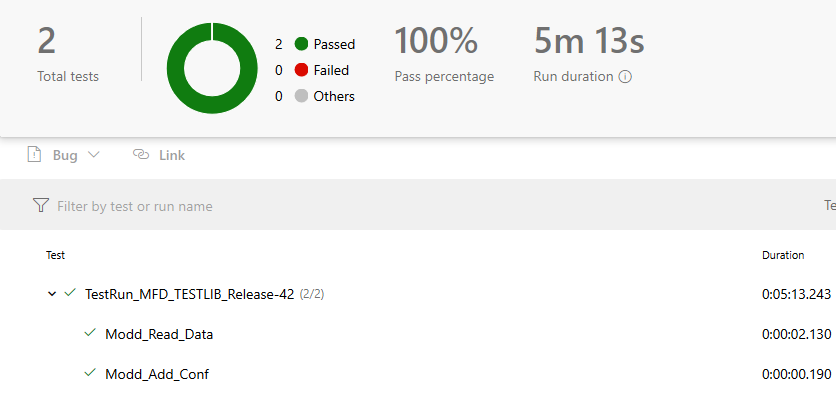
\includegraphics[width=\textwidth]{assets/img/azure.png}
    \caption{Snímek ze serveru Azure DevOps s výsledky testů}
    \source{Azure DevOps Server \cite{azure_devops_software}}
    \label{fig:azure}
\end{figure}

Po dokončení testu můžeme zobrazit i protokol běhu testovací služby. Protokol je vytvořen v kořenové složce zkompilovaného testovacího projektu, tedy ve složce, ze které je testování spouštěno. Nejjednodušším způsobem, jak tento soubor zobrazit, je vypsáním jeho obsahu skrz příkazovou řádku. Zároveň lze vytvořit pravidlo, aby byl tento protokol vypisován pouze v případě neúspěchu nějakého z testů. Výpis protokolu z demonstrativního testovacího běhu můžeme vidět na výpisu \ref{listing:run_log}.

\begin{listing}[p]
    \centering
    \begin{minted}[breaklines,autogobble, fontsize=\footnotesize]{cpp}
class TestModdReadData : public ITestCase {
public:
    bool StartUp() {
        NV_IP_SUITE* pIpSuite;
        MFD_INT len;
        MFD_IP_SUITE networkInfo;
        MFD_AlignPack alignPack = MFD_ALIGN_PACK_1;

        // Configuration of ModbusTCP
        if ((mfd_modd_add_configuration(1, 0, 4, 2, 0, alignPack, MFD_MODULE_STANDARD)) != MFD_TRUE) { 
            return false; 
        }

        // Restore network information from memory
        Bsp_nv_data_restore(PNIO_NVDATA_IPSUITE, (PNIO_VOID**)&pIpSuite, (PNIO_UINT32*)&len);
        networkInfo.ipAddress = LSA_HTONL(pIpSuite->IpAddr);
        networkInfo.ipMask = LSA_HTONL(pIpSuite->SubnetMask);
        networkInfo.ipGateway = LSA_HTONL(pIpSuite->DefRouter);

        // ModbusTCP inicialization
        if (mfd_modd_online(&networkInfo) != MFD_TRUE) {
            return false;
        }

        if (mfd_modd_start() != MFD_TRUE) {
            return false;
        }
            
        // Set output data
        MFD_BYTE* data;
        MFD_BYTE control_data[8] = { 0,0xDE,0,0xAD,0,0xBE,0,0xEF };
            
        mfd_modd_out_data_lock(const_cast<const MFD_BYTE**>(&data));
        MFD_MEMCPY(data, control_data, 8);
        return mfd_modd_out_data_unlock() == MFD_TRUE;
    }

    bool Test() {
        return true;
    }

    bool TearDown() {
        return mfd_modd_stop() == MFD_TRUE && mfd_modd_offline() == MFD_TRUE && mfd_modd_remove_configurations() == MFD_TRUE;
    }
};
    \end{minted}
\caption{Implementace testu na testovaném zařízení}
\label{listing:testcase_device}
\end{listing}


\begin{listing}[p]
    \centering
    \begin{minted}[breaklines,autogobble, fontsize=\footnotesize]{csharp}
class TestModdReadData : ITestCase
{
    public bool StartUp()
    {
        return true;
    }

    public bool Test()
    {
        // Get IP address of test device
        IPAddress devkit;
        if (!API.GetParticipantIp(PhysicalAddress.Parse("080006020110"), out devkit))
            return false;

        // Create ModbusTCP connection
        client = new ModbusClient(devkit.ToString(), 502);

        try 
        {
            client.Connect();
        }
        catch 
        {
            return false;
        }

        if (!client.Connected)
            return false;

        // Read data from device
        var test = client.ReadHoldingRegisters(0, 4);
            
        // Compare to expected data
        int[] controlData = { 0xDE, 0xAD, 0xBE, 0xEF };
        return Enumerable.SequenceEqual(controlData, test);
        }


    public bool TearDown()
    {
        client.Disconnect();
        return true;
    }

    ModbusClient client;
}
    \end{minted}
\caption{Implementace testu pro testovacího partnera}
\label{listing:testcase_partner}
\end{listing}

\begin{listing}[p]
    \centering
    \begin{minted}[breaklines,fontsize=\footnotesize]{csharp}
[TestClass]
public class Modbus
{
    [TestMethod]
    public void TestModdAddConf()
    {
        API.Run(TestCaseE.MODD_ADD_CFG);
    }
    
    [TestMethod]
    public void TestModdReadData()
    {
        for (int x = 0; x < 8; x++)
            API.AddTestPartner(new TestLib.Client.TestPartner(new TestModdReadData()));
    
        API.Run(TestCaseE.MODD_READ_DATA);
    }
    
}
    \end{minted}
\caption{Implementace testů v testovacím projektu}
\label{listing:testcase_service}
\end{listing}


\begin{listing}[p]
    \centering
    \begin{minted}[breaklines,fontsize=\footnotesize]{text}
[4.5.21 - 14:55:26] Server ready on 192.168.0.15:1337
[4.5.21 - 14:55:26] Expected physical participants: 1
[4.5.21 - 14:55:35] Device with MAC address 080006020110 connected
[4.5.21 - 14:55:35] All devices connected, starting tests
[4.5.21 - 14:55:35] Running test: MODD_ADD_CFG
[4.5.21 - 14:55:35] Test successful
[4.5.21 - 14:55:35] Test partner connected
[4.5.21 - 14:55:36] Test partner connected
[4.5.21 - 14:55:36] Test partner connected
[4.5.21 - 14:55:36] Test partner connected
[4.5.21 - 14:55:36] Test partner connected
[4.5.21 - 14:55:36] Test partner connected
[4.5.21 - 14:55:36] Test partner connected
[4.5.21 - 14:55:36] Test partner connected
[4.5.21 - 14:55:36] Running test: MODD_READ_DATA
[4.5.21 - 14:55:38] Test successful
[4.5.21 - 14:55:38] Test partner disconnected
[4.5.21 - 14:55:38] Test partner disconnected
[4.5.21 - 14:55:38] Test partner disconnected
[4.5.21 - 14:55:38] Test partner disconnected
[4.5.21 - 14:55:38] Test partner disconnected
[4.5.21 - 14:55:38] Test partner disconnected
[4.5.21 - 14:55:38] Test partner disconnected
[4.5.21 - 14:55:38] Test partner disconnected
[4.5.21 - 14:55:38] Run finnished, all tests finnished successfully
    \end{minted}
    \caption{Záznam provedeného testovací běhu}
    \label{listing:run_log}
\end{listing}